\documentclass[11pt,a4paper]{article}

\usepackage[utf8]{inputenc}
\usepackage[T1]{fontenc}
\usepackage{lmodern}
\usepackage[spanish,es-nodecimaldot]{babel}
\usepackage[a4paper,margin=2.2cm]{geometry}
\usepackage{booktabs}
\usepackage{graphicx}
\usepackage{array}
\usepackage{longtable}
\usepackage{enumitem}
\usepackage{xcolor}
\usepackage{listings}
\usepackage{tikz}
\usetikzlibrary{arrows.meta,positioning,shapes.geometric}
\usepackage[hidelinks]{hyperref}
\usepackage{microtype}

\definecolor{codegray}{gray}{0.95}
\lstset{
  basicstyle=\ttfamily\small,
  backgroundcolor=\color{codegray},
  frame=single,
  breaklines=true,
  columns=fullflexible,
  keepspaces=true
}

\title{Extractor de facturas FEL con LLM}
\author{Angel Esteban Esquit Hernández \and Javier Eduardo España Pacheco\\CC3092 Deep Learning y Sistemas Inteligentes}
\date{Proyecto 3 -- Entrega: 6 de noviembre de 2026}

\begin{document}
\maketitle
\tableofcontents
\newpage
\setcounter{section}{2}

\subsection{Problema y usuario}
Las pymes y los equipos contables reciben facturas en PDF o imagen con layouts, idiomas, monedas y etiquetas diferentes. La digitación manual en una hoja de cálculo es repetitiva y las reglas por proveedor no escalan. El producto recibe una factura y devuelve un JSON/CSV revisable con los campos principales de una factura FEL.

El usuario objetivo es un contador o auxiliar administrativo que necesita registrar facturas con rapidez, pero debe conservar revisión humana antes de usar los datos en contabilidad oficial. El sistema no sustituye una validación tributaria ni una aprobación contable.

\subsection{Producto y arquitectura}
El flujo del producto es:
\begin{enumerate}
  \item El usuario sube un PDF, PNG, JPG o WEBP desde Streamlit.
  \item El extractor lo convierte en una entrada multimodal y solicita una salida estructurada \texttt{Factura} con Pydantic.
  \item Los validadores revisan IVA, sumas, líneas, NIT, fecha y UUID.
  \item Si hay inconsistencias, se puede hacer un único reintento con los problemas explícitos.
  \item La interfaz muestra campos y advertencias, y permite descargar JSON y CSV.
\end{enumerate}

\begin{figure}[ht]
\centering
\begin{tikzpicture}[
  node distance=8mm and 12mm,
  box/.style={draw, rounded corners, align=center, minimum height=9mm, minimum width=27mm},
  decision/.style={draw, diamond, align=center, aspect=2, inner sep=1pt},
  arrow/.style={-{Latex[length=2mm]}, thick}
]
  \node[box] (input) at (0,0) {PDF o imagen};
  \node[box] (multi) at (38mm,0) {Entrada\\multimodal};
  \node[decision] (model) at (76mm,0) {Modelo};
  \node[box] (openai) at (118mm,8mm) {OpenAI\\Responses};
  \node[box] (anthropic) at (118mm,-8mm) {Anthropic\\Messages};
  \node[box] (schema) at (118mm,-32mm) {Factura\\Pydantic};
  \node[box] (valid) at (76mm,-32mm) {Validadores\\deterministas};
  \node[box] (ui) at (38mm,-32mm) {Streamlit};
  \node[box] (download) at (76mm,-50mm) {JSON / CSV};
  \draw[arrow] (input) -- (multi);
  \draw[arrow] (multi) -- (model);
  \draw[arrow] (model) -- (openai);
  \draw[arrow] (model) -- (anthropic);
  \draw[arrow] (openai.east) -- ++(6mm,0) |- (schema.east);
  \draw[arrow] (anthropic.south) -- (schema.north);
  \draw[arrow] (schema) -- (valid);
  \draw[arrow] (valid) -- (ui);
  \draw[arrow] (valid) -- (download);
  \draw[arrow] (valid.north) -- node[right, font=\scriptsize, align=left]{m\'aximo 1\\reintento} (model.south);
\end{tikzpicture}
\caption{Arquitectura del extractor.}
\end{figure}

No se usa RAG ni embeddings: la tarea es extracción de un documento individual y no recuperación de conocimiento. La generación se limita a 2.000 tokens; las comparaciones de este informe usan cero reintentos para controlar costo.

\subsection{Datos}
\subsubsection{FEL sintético}
El conjunto principal contiene 45 documentos generados con semilla 2026 por \texttt{scripts/make\_synthetic.py}. Incluye cuatro layouts, PDFs e imágenes, fechas en tres formatos, una a ocho líneas, ruido, rotación, desenfoque y facturas de pequeño contribuyente sin IVA.

Durante la revisión se corrigió un error de etiquetado: seis facturas sin IVA tenían \texttt{subtotal} igual al total aunque el documento no lo mostraba. El gold corregido usa \texttt{subtotal: null} y se regeneraron los seis JSON afectados. La corrección se documenta como error de etiquetado, no como ajuste de una predicción.

\subsubsection{Dataset público adicional}
Se integraron 15 fixtures sintéticas del \href{https://github.com/SalorWorks/shopify-invoice-test-pack}{Synthetic Shopify Invoice Test Pack}, con licencia CC BY 4.0. Cada caso conserva PDF y PNG y tiene una referencia convertida al esquema local. Incluye multipágina, árabe, bilingüe, descuentos, flete, duty, mala calidad y tablas densas.

Este conjunto es una prueba de robustez y no representa facturas FEL guatemaltecas: sus campos fiscales, monedas y estructura comercial son distintos. No se presentan como facturas reales ni como validación tributaria.

\subsection{Modelos y técnica}
Se compararon tres modelos multimodales con salida estructurada:
\begin{itemize}
  \item \texttt{gpt-4o-mini}, mediante OpenAI Responses API.
  \item \texttt{claude-haiku-5-5}, mediante Anthropic Messages API.
  \item \texttt{claude-sonnet-5-5}, mediante Anthropic Messages API.
\end{itemize}

La técnica combina prompting, esquema Pydantic, validación determinista y retroalimentación opcional. No se hizo fine-tuning. El prompt v1 es mínimo; v2 especifica nulos, normalización, fechas, montos y defensa contra instrucciones incrustadas en el documento.

\subsection{Evaluación}
Se midió exactitud por campo, porcentaje de documentos completamente correctos, salida válida, latencia, tokens y costo estimado. El baseline es regex sobre texto de PDF y no procesa imágenes.

\subsubsection{Resultados FEL, 45 documentos}
\begin{table}[ht]
\centering
\caption{Comparación principal sin reintentos.}
\begin{tabular}{lrrrr}
\toprule
Sistema & Exactitud & Docs. 100\% & Latencia & Costo/doc. \\
\midrule
Regex & 23,25\% & 0\% & -- & USD 0 \\
GPT-4o-mini & 90,77\% & 15,56\% & 4,923 s & USD 0,00147 \\
Claude Haiku 5.5 & 100\% & 100\% & 5,305 s & USD 0,00076 \\
Claude Sonnet 5.5 & 98,63\% & 82,22\% & 3,958 s & USD 0,0113 \\
\bottomrule
\end{tabular}
\end{table}

El costo total de las tres corridas LLM fue aproximadamente USD 0,6084. Haiku fue la mejor relación precisión/costo en este conjunto. Sonnet no justificó su costo adicional.

\subsubsection{Resultados públicos, 15 documentos}
\begin{table}[ht]
\centering
\caption{Comparación sobre el dataset público.}
\begin{tabular}{lrrrr}
\toprule
Sistema & Exactitud & Docs. 100\% & Latencia & Costo/doc. \\
\midrule
GPT-4o-mini & 72,31\% & 0\% & 3,657 s & USD 0,00155 \\
Claude Haiku 5.5 & 83,08\% & 6,67\% & 4,120 s & USD 0,00078 \\
Claude Sonnet 5.5 & 91,28\% & 33,33\% & 3,601 s & USD 0,01162 \\
\bottomrule
\end{tabular}
\end{table}

En este conjunto Sonnet obtuvo el mejor resultado, seguido por Haiku y GPT. Las principales diferencias aparecen en nombres, NIT y líneas, porque el dataset usa un esquema comercial internacional distinto al FEL local. Esto confirma que la ventaja de Haiku en el conjunto FEL no es universal: depende del dominio y de la distribución de los documentos.

\subsection{Experiencia de usuario}
La aplicación Streamlit ofrece:
\begin{itemize}
  \item Selector de modelo y reintentos de corrección.
  \item Validación de la clave del proveedor seleccionado.
  \item Límite de archivo de 10 MB y validación de extensión.
  \item Tabla de campos generales y líneas.
  \item Advertencias de validadores para revisión humana.
  \item Descarga de JSON y CSV.
  \item Latencia, tokens, costo estimado e intentos visibles.
\end{itemize}

\begin{figure}[ht]
\centering
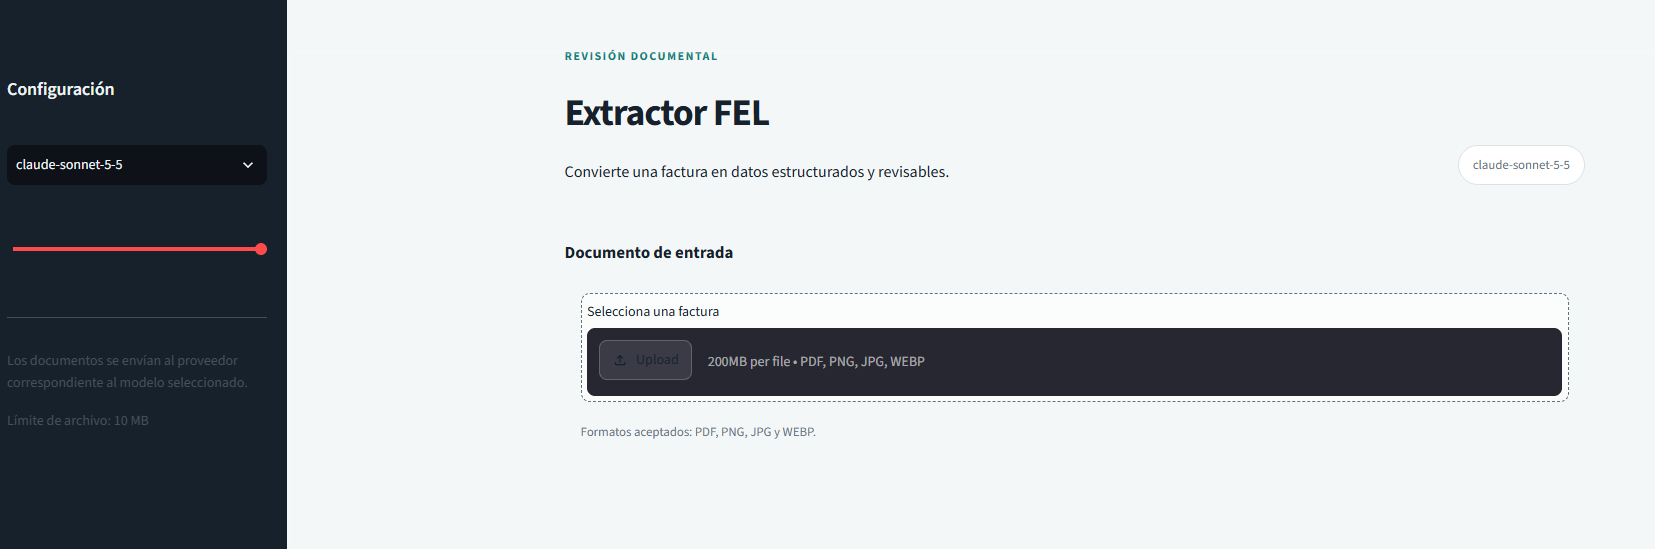
\includegraphics[width=\linewidth]{img/Captura1.png}
\caption{Pantalla inicial: selector de modelo, aviso de privacidad y carga de la factura (PDF, PNG, JPG o WEBP).}
\end{figure}

\begin{figure}[ht]
\centering
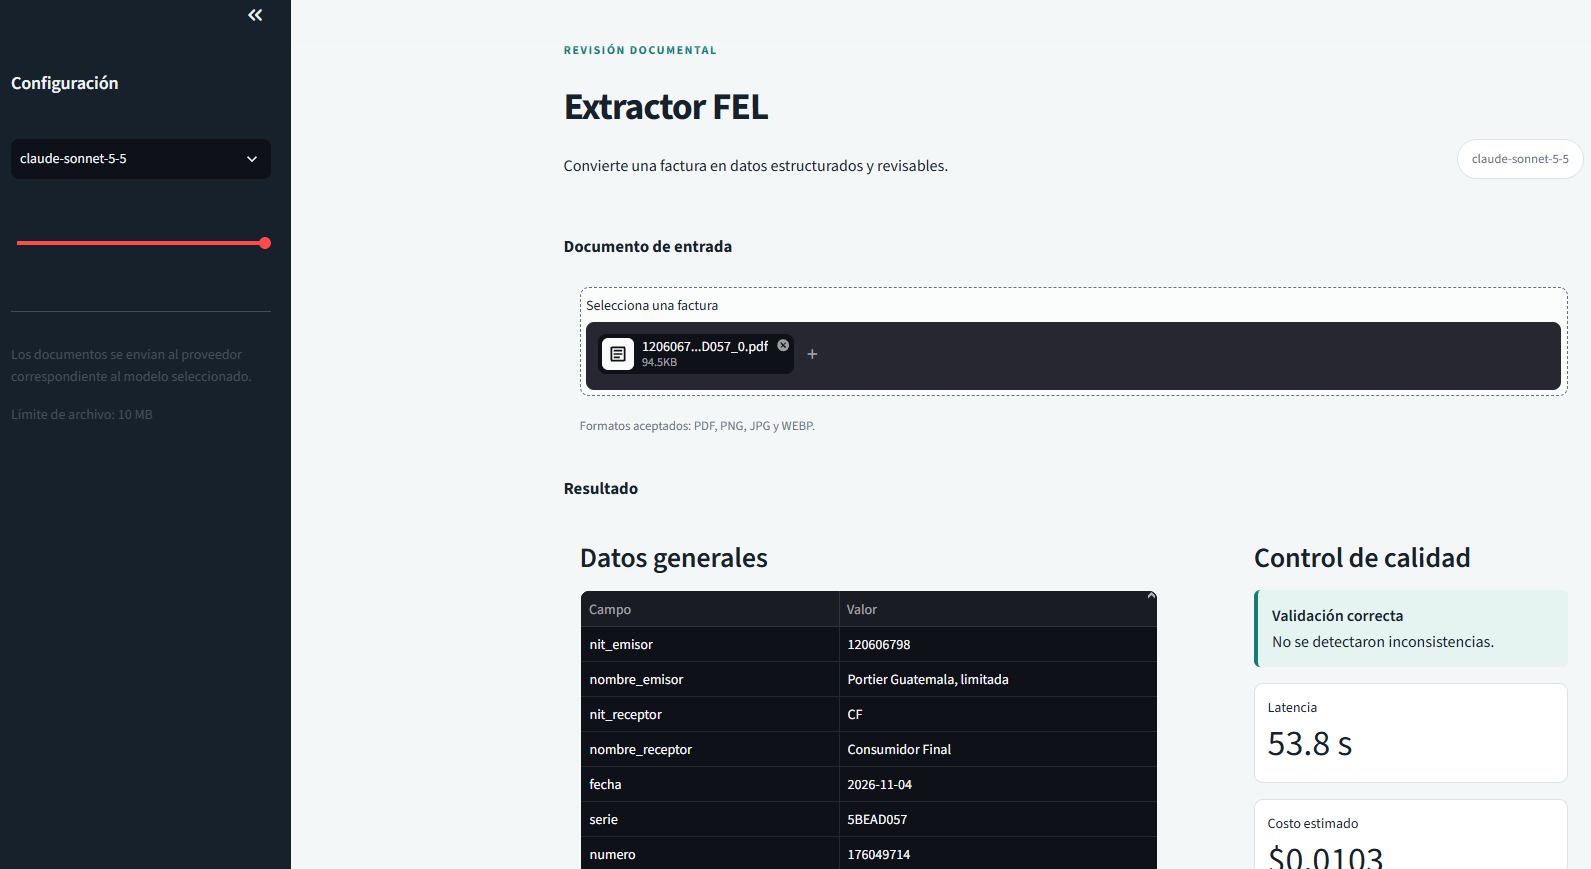
\includegraphics[width=\linewidth]{img/Captura2.png}
\caption{Factura cargada y resultado: datos generales extraídos, control de calidad (``Validación correcta''), latencia y costo estimado.}
\end{figure}

\begin{figure}[ht]
\centering
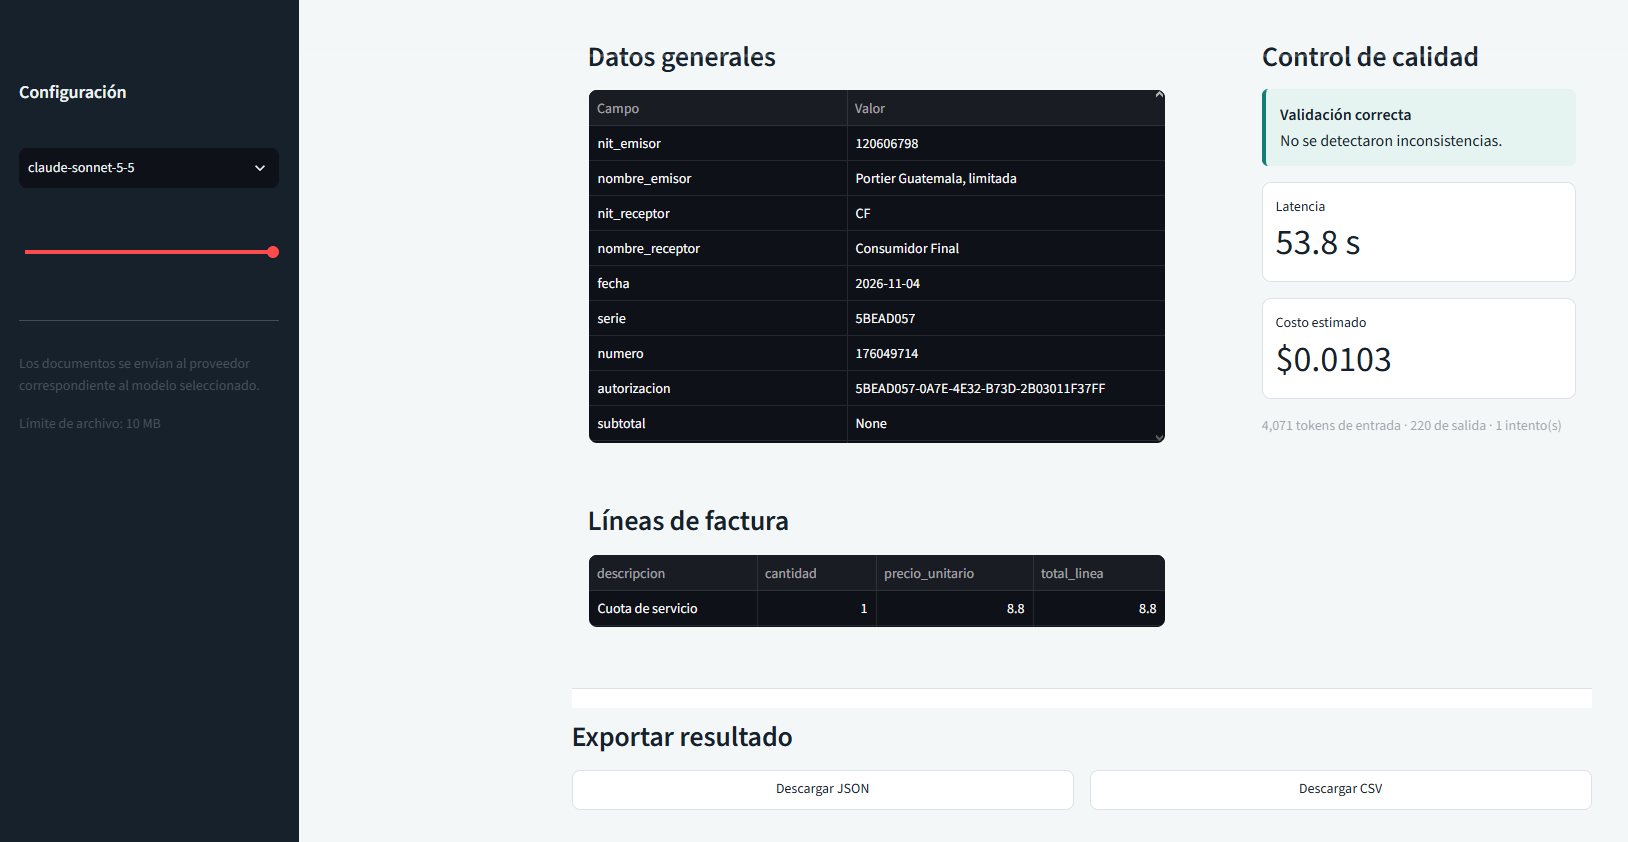
\includegraphics[width=\linewidth]{img/Captura3.png}
\caption{Resto del resultado: líneas de factura, tokens e intentos, y botones para exportar JSON y CSV. El campo \texttt{subtotal} aparece como \texttt{None} porque el documento no lo muestra.}
\end{figure}

La latencia de la Figura 2 (53,8 s) es una sola medición de la interfaz y es mucho mayor que el promedio de 3,96 s de Sonnet en la evaluación por lotes; puede deberse a la primera llamada o a la red, y no se tomó como representativa.

La interfaz no debe usarse como aprobación automática: el resultado siempre requiere revisión cuando hay advertencias o cuando el documento contiene conceptos que el esquema no modela, como descuentos, flete o duty.

\subsubsection{Prueba de usabilidad}
Se pidió a personas ajenas al grupo, sin ayuda, que (1) subieran una factura y obtuvieran el JSON o CSV, (2) identificaran qué campo quedó marcado para revisión y por qué, y (3) corrigieran un valor. Se registró si completaron cada tarea, el tiempo, dónde dudaron, una calificación de facilidad de 1 a 5 y un comentario.

\begin{table}[ht]
\centering
\caption{Resultados de la prueba de usabilidad (completar con datos observados).}
\begin{tabular}{lcccccc}
\toprule
Tester & Tarea 1 & Tarea 2 & Tarea 3 & Tiempo & Facilidad (1--5) & Comentario \\
\midrule
 &  &  &  &  &  &  \\
 &  &  &  &  &  &  \\
 &  &  &  &  &  &  \\
\bottomrule
\end{tabular}
\end{table}

\subsection{Riesgos, privacidad y limitaciones}
Los documentos se envían al proveedor correspondiente al modelo seleccionado. No se deben subir facturas que no puedan compartirse con OpenAI o Anthropic. Las claves viven únicamente en \texttt{.env}, excluido de Git.

El documento se trata como dato y el prompt ordena ignorar instrucciones contenidas en la factura. Esto reduce prompt injection, pero no elimina errores de interpretación. Los validadores detectan inconsistencias, no garantizan exactitud fiscal.

El conjunto principal es sintético y fue creado por el mismo equipo que diseñó el extractor. El conjunto público también es sintético y no reemplaza datos reales anonimizados del flujo de trabajo. El algoritmo del NIT, los campos FEL y el supuesto de IVA deben contrastarse con documentación oficial antes de producción.

\subsection{Conclusiones y trabajo futuro}
El producto es funcional y reproducible para demostración y evaluación controlada. Haiku 5.5 es la configuración recomendada por su resultado y costo. GPT-4o-mini es una alternativa de bajo costo, aunque perdió precisión en el conjunto FEL. Sonnet ofrece buen desempeño, pero con un costo aproximadamente quince veces mayor que Haiku en esta corrida.

El siguiente trabajo es añadir facturas reales anonimizadas con permiso, revisión cruzada de sus gold, prueba de usabilidad con usuarios externos, capturas, video de demostración y validación formal de supuestos tributarios. Esos elementos no se deben inventar a partir de datasets sintéticos.

\subsection{Reproducibilidad y repositorio}
Repositorio de GitHub: \url{https://github.com/Javier-Espana/PRY3-DL}

\begin{lstlisting}[language=bash]
python3 -m venv .venv
.venv/bin/python -m pip install -r requirements.txt
cp .env.example .env
.venv/bin/python -m pytest -q
.venv/bin/python -m streamlit run src/app.py
\end{lstlisting}

Para repetir las métricas FEL:
\begin{lstlisting}[language=bash]
.venv/bin/python -m src.evaluate --system regex
.venv/bin/python -m src.evaluate --system llm --model gpt-4o-mini --prompt v2 --retries 0
.venv/bin/python -m src.evaluate --system llm --model claude-haiku-5-5 --prompt v2 --retries 0
.venv/bin/python -m src.evaluate --system llm --model claude-sonnet-5-5 --prompt v2 --retries 0
\end{lstlisting}

Para el dataset público:
\begin{lstlisting}[language=bash]
.venv/bin/python -m src.evaluate --system llm --model claude-haiku-5-5 \
  --prompt v2 --retries 0 --docs data/public/shopify/docs \
  --gold data/public/shopify/gold --run-name public_shopify
\end{lstlisting}

\begin{thebibliography}{9}
\bibitem{shopify}
SalorWorks, \emph{Synthetic Shopify Invoice Test Pack}, CC BY 4.0, 2026.\\
\url{https://github.com/SalorWorks/shopify-invoice-test-pack}

\bibitem{fatura}
M. Limam, M. Dhiaf y Y. Kessentini, \emph{FATURA Dataset}, Zenodo, 2023.\\
\url{https://zenodo.org/records/8261508}
\end{thebibliography}

\end{document}
